\documentclass{article}
% basics
\usepackage{amsfonts}
\usepackage{enumitem}
\usepackage{float}
\usepackage{graphicx}
\usepackage{hyperref} 
\usepackage[labelfont=bf]{caption}

\newtheorem{theorem}{Theorem}
\newtheorem{lemma}[theorem]{Lemma}
\newtheorem{corollary}{Corollary}[theorem]

% unique math expressions:  
\usepackage{amsmath}
\DeclareMathOperator*{\andloop}{\wedge}
\DeclareMathOperator*{\pr}{Pr}
\DeclareMathOperator*{\approach}{\longrightarrow}
\DeclareMathOperator*{\eq}{=}

% grey paper
\usepackage{xcolor}
% \pagecolor[rgb]{0.11,0.11,0.11}
% \color{white}

% embedded code sections
\usepackage{listings}
\definecolor{codegreen}{rgb}{0,0.6,0}
\definecolor{codegray}{rgb}{0.5,0.5,0.5}
\definecolor{codepurple}{rgb}{0.58,0,0.82}
\lstdefinestyle{mystyle}{
    commentstyle=\color{codegreen},
    keywordstyle=\color{magenta},
    numberstyle=\tiny\color{codegray},
    stringstyle=\color{codepurple},
    basicstyle=\ttfamily\footnotesize,
    breakatwhitespace=false,         
    breaklines=true,                 
    captionpos=b,                    
    keepspaces=true,                 
    numbers=left,                    
    numbersep=5pt,                  
    showspaces=false,                
    showstringspaces=false,
    showtabs=false,                  
    tabsize=2
}

\lstset{style=mystyle}

\begin{document}
\author{Yosef Goren \& Ori Evron}
\title{Internet Networking - Homework 5}
\maketitle
\tableofcontents

\section{Max/Min Fairness}
\subsection{Splitting the problem}
First we note that we can segnificantly simplify the solution by splitting
the problem into two distinct parts: Since there is no contention
between the flows which go clockwise and those that go counter-clockwise,
we can address each of these classes separatly - and the combined results
will be equivalent to if we were to run the algorithm separatly on each one.

\subsection{Clockwise Flows}
In the fisrt round, we see that the link betweenn node 3 and 4 is the bottleneck.
this happans because as seen in the graph, the number of flows that passes it is maximal,
so, all the passing flows have a valeu of 1/6.
In the second round, all the flows that passes through the lin between 3 and 4 are removed,
and the new bottleneck is the link between nodes 5 and 6, the flow  between 5 to 6 and 4 to 6 each get 1/4.
In the thierd round, the only flow left is the flow beween 4 to 5, it has 10 - 5/6 - 1/4 = 8 + 11/12.\\
The details can also seen in the attached photo:\\
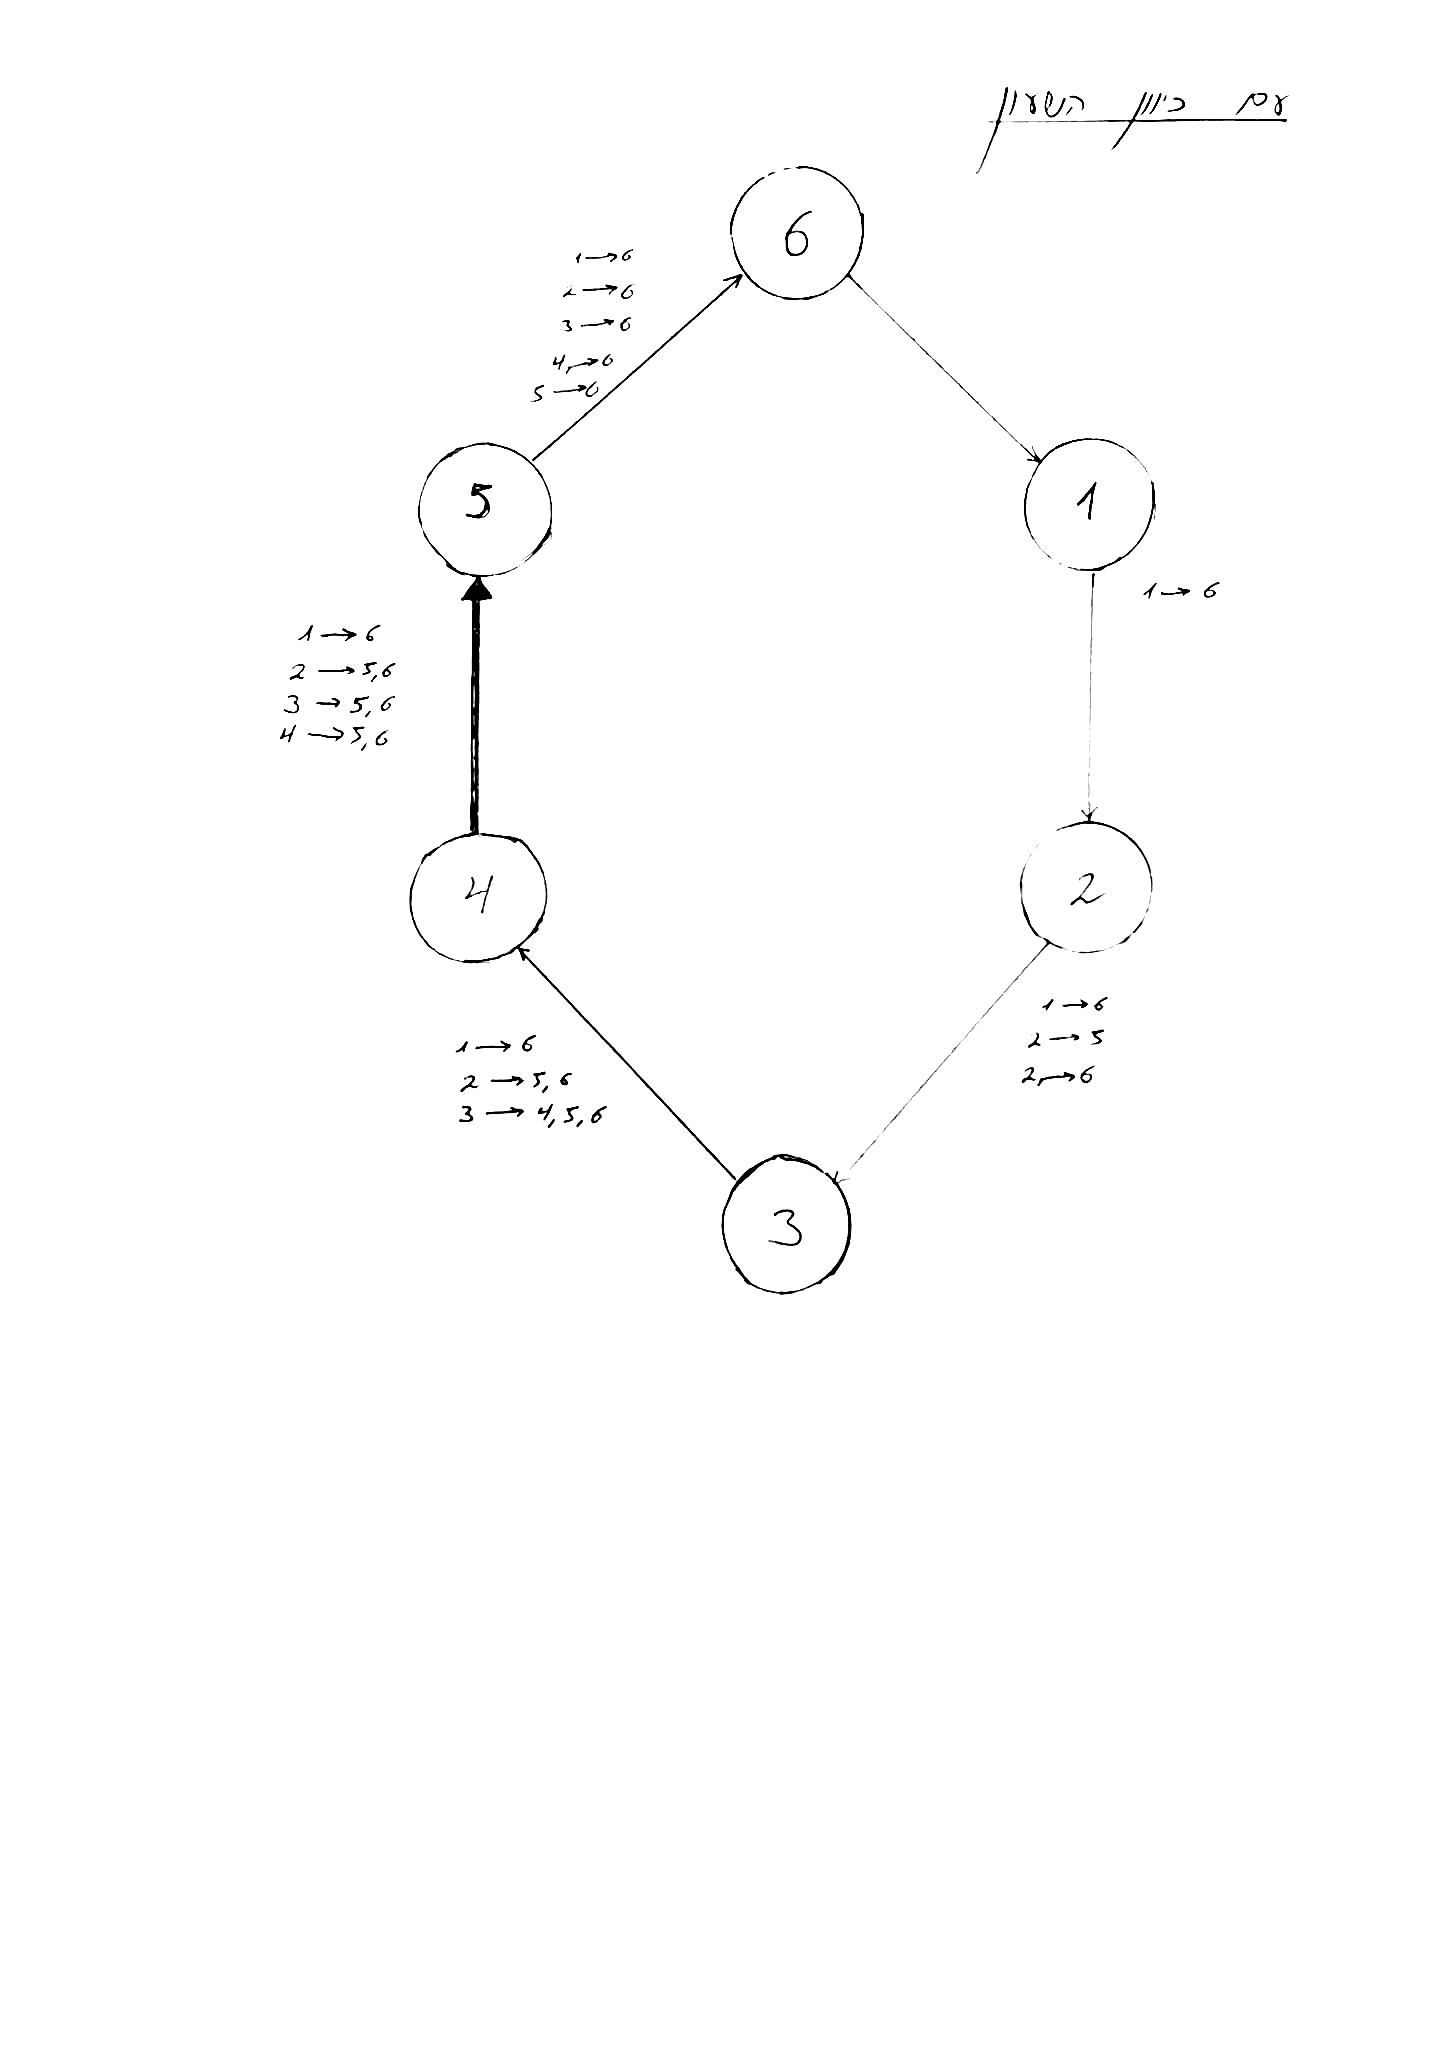
\includegraphics[width=\textwidth]{i2.png}

\subsection{Counter-Clockwise Flows}
In the first round, we see that the link with the minimal
allocatable bandwidth per flow (a.k.a the bottleneck) is the link from
2 to 1 - which has 8 flows contending for it's bandwith, while it can only
pass 1 unit - meaning each flow will only recive $\frac{1}{8}$ of a unit.\\
At this point - we can eliminate all flows involved in that link - 
which leaves us with a single flow from node 1 to node 6.
Note that the bandwidth left on that link is now 9. This link is also
the next bottleneck. Hence the $1\rightarrow 6$ flow recived 9 bandwidth units
in total - and all flows have been eliminated.\\
To sum up the final bandwidths recived by each flow:
\begin{itemize}
    \item $1\rightarrow 6$: 9 units of bandwidth.
    \item All ofther flows: $\frac{1}{8}$ units of bandwidth.
\end{itemize}
The details can also seen in the attached photo:\\
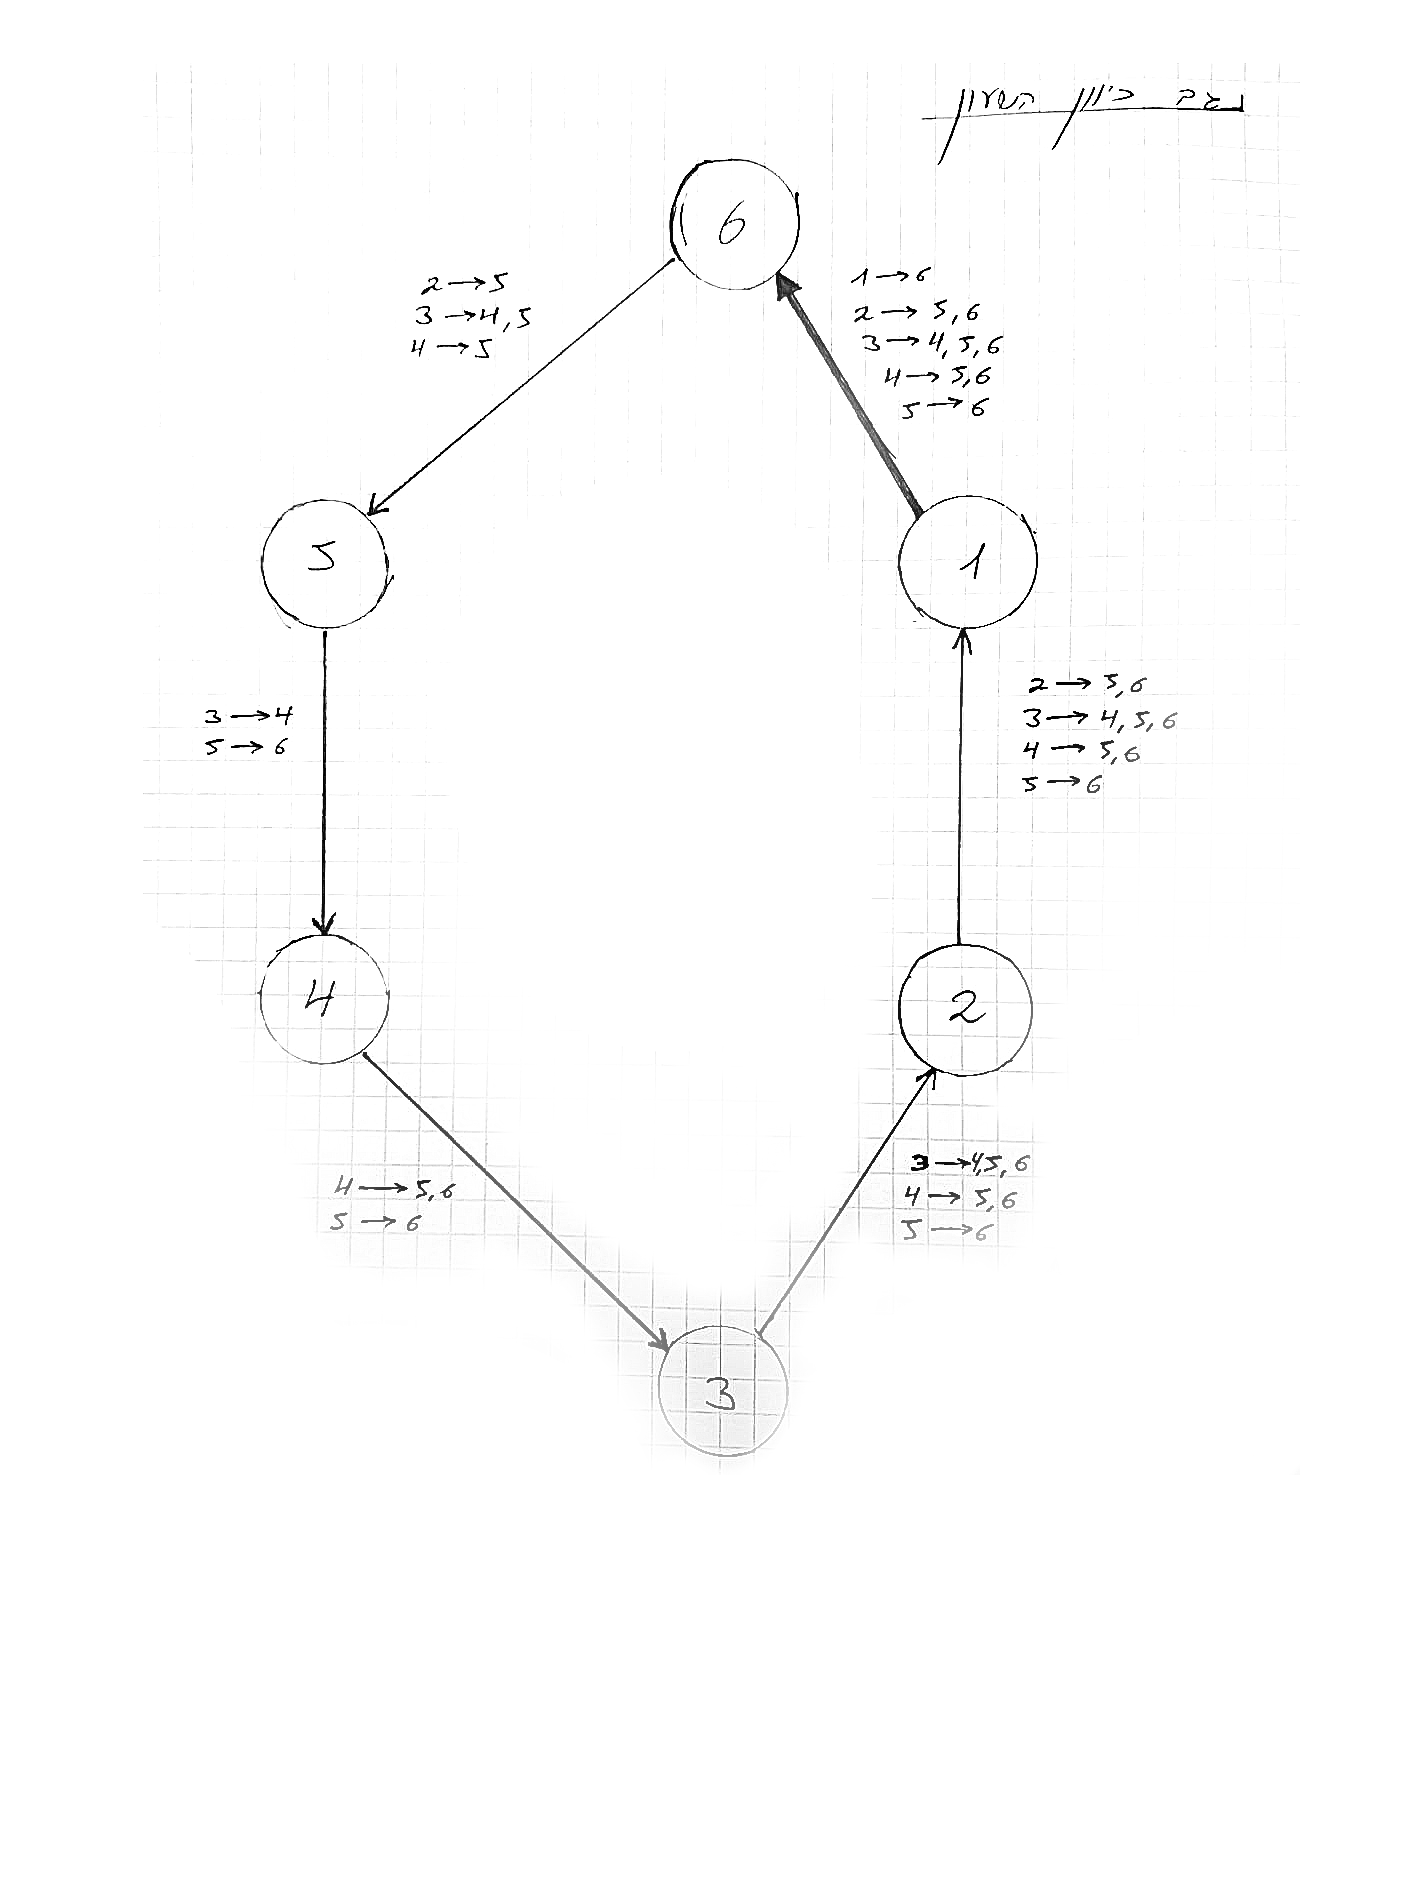
\includegraphics[width=\textwidth]{i1.png}


\section{TCP Reno Congestion Control}
\subsection{}
The Transmission rounds where the \texttt{ssthresh} value
changes are the ones where a drop is seen due to a duplicate ack:
rounds 16 and 22. After round 16 - \texttt{ssthresh} is set to 21 segments
and after round 22 it is set to about 13 segments.

\subsection{}
The time intervals during which the algorithm operates in "slow start"
are between 0 and 6, and from 23 until the end.

\subsection{}
This would cause \texttt{cwnd} and \texttt{ssthresh}
to drop to about 4 segments.

\subsection{}
After the 16th round, the packet loss was detected through duplicate ACKs.
This conclusion is supported by the fact that the congestion window (cwnd) was not set to 1.\\
If the case were a timeout, the cwnd would have been set to 1.


\subsection{}
The round 22 packet loss was discovered by a timout. We know this is
the case due to the way \texttt{cwnd} has changed: since it drops
directly to 1 instead of halfing it's value - we know it was a timeout.

\subsection{}
The initial value for \texttt{ssthresh} was 32 or 33,
we know this since this is the point where the congestion control
policy changes from slow start to congestion avoidance.

\subsection{}
By essentially doing an integral over the graph we can find
how many segmests have been sent up to a certain point. Since we want to
know when the 100'th segment was sent - we apply this proccess up to the point
where the accumulating integral is equal to 100.
After transmission round the total is 63,
and after transmission round the total is 126
- so the 100'th segment must have been sent at the 7'th round.

\section{TCP Congestion Control}
\subsection{}
According to Tutorial 8, the only way for TCP Reno and TCP New Reno to detect congestion is by creating it.
This means increasing the congestion window (cwnd) and waiting for a packet loss.
The main differences between TCP Reno and TCP New Reno are
New Reno's use of Selective Acknowledgment (SACK) and the modified fast recovery.

\subsection{}
TCP Vegas detects congestion by estimating the optimal throughput.
It calculates the throughput and compares it to the current throughput minus alpha.
If the current throughput is greater, TCP Vegas assumes there
is congestion and lowers the packet sending speed.

\subsection{}
Contrary to TCP Reno, TCP Vegas does not divide the congestion window (cwnd) in half when congestion is detected.
Instead, TCP Vegas lowers the cwnd size in a linear manner. This approach minimizes the impact on throughput compared to TCP Reno,
as it avoids the "saw" shape in the cwnd as a function of time graph.

\subsection{}
TCP Vegas can be outperformed by TCP Reno. This is because, during the initial stages,
TCP Vegas lacks a slow start phase. As a result, the increase in congestion window (cwnd) of TCP Vegas is linear,
whereas TCP Reno exhibits an exponential increase.

\subsection{}
TCP Compound maintains two types of windows: the original congestion window (cwnd) and the delay window (dwnd).
It uses both dwnd and cwnd to calculate the sending window. The dwnd represents the delay component of CTCP,
and by utilizing dwnd, CTCP can achieve better scalability in high-speed and long-delay networks.

\subsection{}
The protocol can lower the congestion window (cwnd) in a linear manner instead of dividing it in half,
resulting in a better throughput.

\subsection{}
The protocol has additional variables, such as the delay variable,
which it can use to calculate the estimated throughput more accurately compared to TCP Vegas.



% \section{TCP Cubic Congestion Control}

\end{document}